% !TeX spellcheck = en_GB 
\documentclass[a4paper, 11pt, headings=standardclasses, tablecaptionsbelow]{scrartcl}

\usepackage[margin=2.5cm]{geometry}
\usepackage{etoolbox}
\usepackage{authblk}
\renewcommand{\Affilfont}{\small}
\newcommand\blfootnote[1]{%
  \begingroup
  \renewcommand\thefootnote{}\footnote{#1}%
  \addtocounter{footnote}{-1}%
  \endgroup
}
\usepackage[style=apa, backend=biber, sorting=ynt, useprefix=true]{biblatex}
\addbibresource{mainstream.bib}
\usepackage[autostyle=false, style=english]{csquotes}
\MakeOuterQuote{"}
\usepackage[british]{babel}
\usepackage[modulo]{lineno}
\linenumbers
\usepackage{appendix}
\usepackage{lscape}
\usepackage[hidelinks]{hyperref}
\usepackage[font=small]{caption}
\usepackage{graphicx}
\usepackage{booktabs}
\usepackage{tabularx}
\newcolumntype{Y}{>{\raggedright\arraybackslash}X}
\newcolumntype{s}{>{\raggedright\arraybackslash\hsize=.5\hsize}X}
\AtBeginEnvironment{tabularx}{\small}
\usepackage{xltabular}
\AtBeginEnvironment{xltabular}{\small}

\title{How is the Mainstream changed? \let\thefootnote\relax\footnotetext{
  This version is intended to be submitted to the XV ESHET Conference
  
  An updated version of this paper and all the source code and the instructions required to replicate the paper are available at \url{https://github.com/TnTo/mainstream/}
}}
\subtitle{A Topic Model insight}
\author{Michele Ciruzzi\thanks{mciruzzi@uninsubria.it - \url{https://orcid.org/0000-0003-1485-1204}}}

\begin{document}

\maketitle

%\begin{abstract}
%\end{abstract}

\section{Why studying the mainstream?}
To understand the reasons of this work and, eventually, its scientific relevance a premise is necessary.

Economics as discipline presents very strong social norms and a very hierarchical structure.
As result, it is possible, and quite easy, to identify a small group of journals in which the scholars in the top US department often publish \parencite{card2013,kim2006,kim2009,dusansky1998,hamermesh2013,ellison2003,heck2006}.
Those are the same journals that are able to assure a scholar the tenure in the very same departments, by publishing one of their papers \parencite{heckman2020}.

In other words, there is a group of journals (the Top5 or the Blue Ribbon Eight) which are liked (and managed) by those who are generally liked (and cited and funded) by the discipline.

This concentration of power and, as consequence, prestige has, inevitably, created a notion of prestige in every aspect of the discipline: there are more prestigious theories, more prestigious research topics, more prestigious departments and so on.

But it happens quickly, in the underfunded academia, that the most prestigious alternatives became the only alternatives, inducing conformism and, as a matter of necessity, excluding less prestigious theories from scientific debate.

The prestigious economics is, politely, knows as \textit{mainstream economics} or, in a more colourful way, as \textit{orthodox economics}. The idea of an orthodoxy, and so of some competing heterodoxies, move the analysis to the semantic field of religion and faith. And it is wanted.

As many, mostly heterodox, scholars have pointed out, many of the hypotheses which support the mainstream economics have to be accepted by faith, since there are not real-world evidences of their realism\footnote{Some orthodox scholars address this criticism by not considering realism as necessary in a scientific theory, but discussing this would be a too long digression.}.
The consequence is that to pursue a career in economics and be able to get a prestigious (and so well-funded) position, a profession of faith is required to every (young) scholar\footnote{An example of this kind of "religious" reasoning is proposed by Galbraith: \textit{"Accepted in reputable market orthodoxy is, as noted, the inherent perfection of the market. The market can reflect contrived or frivolous wants; it can be subject to monopoly, imperfect competition, or errors of information, but, apart from these, it is intrinsically perfect. Yet clearly the speculative episode, with increases provoking increases, is within the market itself. And so is the culminating crash. Such a thought being theologically unacceptable, it is necessary to search for external influences—in more recent times, the downturn in the summer of 1929, the budget deficit of the 1980s, and the “market mechanisms” that brought the crash of 1987. In the absence of these factors, the market presumably would have remained high and gone on up or declined gently without inflicting pain. In such fashion, the market can be held guiltless as regards inherently compelled error. There is nothing in economic life so willfully misunderstood as the great speculative episode."} \parencite{galbraith1994}}.

The last piece of the puzzle I require to justify this work is the role of economics in the society.

Economics is a social science which influences the kind of politics are realized by the governments. It provides theoretical justification, it carries out the forecasts on the real-world effects of policies, it influences the public debate providing the words to convey different ideas of the economy (and so of the society), helping to move the Overton's window.

In other words, Economics is a scientific discipline with a strong impact on the society, and the social and political implications of any economic theory must not be overlooked\footnote{The conceptual framework provided by Keynes' theories is necessary to historically and politically understand Roosevelt and the European social state of the 50s. Similarly, Margaret Thatcher's and Ronald Reagan's economic reforms would never be realized without the theoretical background provided by Friedman.}.

So, critically studying the most widespread economics is necessary to understand which conceptual framework the discipline is providing to the society to understand the reality, to unveil which cultural and political programme it is (more or less consciously) carried out by the discipline.

Nevertheless, this work only tries to describe the mainstream economics, without arguing on the social consequences of the features highlighted. Which is still a necessary first step.

\section{The interpretative hypotheses}
I'm not the first who try to describe mainstream economics, and neither the first to doing it quantitatively (I review some previous attempts in the next section).

Therefore, I can climb up on the shoulder of other scholars to be guided to what I can look for and which interpretative frameworks I can use.

Two qualitative theories will be the core pieces to guide this work: the \textit{empirical turn} hypothesis and the \textit{mainstream pluralism} hypothesis.

The first lens with which observing the mainstream economics is the progressive shift toward empirical research \parencite{backhouse2000,backhouse2016,backhouse2017,cherrier2022}.
Neoclassical economics, which is the theoretical framework on which mainstream economics is based since the seventies, built its fortune on the ability to provide clear models expressed using a very formal flavour of mathematics, mostly calculus-based.
In more recent times instead, in part as a reaction to the credibility crisis arose after the financial crises of the first decade of the XXI century, econometrics is becoming the standard mathematical tool of analysis and theory-driven models are being replaced by data-driven models.
This empirical turn in the scientific practices of the discipline is moving researchers away from the comprehensive economic models of the past, towards a perilous land in which the only theory is the way in which data are analysed, and every economic insight can come only from data itself.

The second lens is the mainstream pluralism hypothesis \parencite{davis2006,davis2019a,davis2019b,cedrini2018}. It has been observed that the domain of research of economics is widening and the number of different computational and mathematical tools used is increasing\footnote{I want to highlight two factors that have probably helped this shift. The first are the new data-driven methodologies, which are able to deal with a wider range of hypotheses than the neoclassical calculus-based approach \parencite{cherrier2022}. The second one is the return from the imperial conquests of other social sciences \parencite{fourcade2015,marchionatti2017}, which has widened the domains of research and introduced new methodologies, like the laboratory experiments that behavioural economists have learnt from psychology.}. These two tendencies have allowed the emergence of many new fields in the discipline, which are very focused on a particular topic (like environmental or health economics) or on a particular method (like economic complexity or behavioural economics).
Researchers who are specialized in one of these fields rarely engage with the other niches, creating an archipelago of unconnected islands and an appearance of pluralism in economics.
The mainstream pluralism hypothesis states that this process of specialization is not developing pluralism as historically intended in economics (i.e. as a plurality of competing ontological views of the economy and the economics), but rather it is creating a plurality of loosely connected fields which shares a common ancestral set of hypothesis (the neoclassical one) and relax some of them to be able to tackle specific problems, putting themself in continuity rather than in contrast with neoclassical economics\footnote{In this sense they can be viewed as subfields of a wider "post-neoclassical" economics, which aims to improve (or save) the neoclassical approach and legacy, rather than rebuild the discipline on completely different assumptions like the heterodoxies aim to do.}.

In the quantitative exercise that constitute the core of this paper, I try to find some evidences in favour of these two hypotheses.

\section{Distant Reading and quantitative methods in the History of Economic Thought}
A common problem in the study of the history of ideas (of which the history of economic thought is surely part) is the impossibility to accurately read a big number of textual documents in a reasonable time. A first, and often adopted, solution is to select a sample of relevant works, like the books of a single author or a handful of representative masterpieces of a period, and analyse only them.
An alternative approach is what Franco Moretti called Distant Reading \parencite{moretti2013}: instead of carefully (close) reading few works, a big number of documents are summarily analysed using statistical methods and the aid of computers.
Different features of a text can be analysed, but generally the focus is on the textual content of the document (recovered by a digital version or through OCRing) or some metadata (title, citations, authors' list).

The kind of data used and the research questions tackled move Distant Reading close to bibliometrics and text mining studies. The fil rouge which ties together Distant Reading studies is their motivation: overcome with quantitative techniques the impossibility to (close) read thousands of document to reconstruct the history of some idea.

The history of neoclassical economics as mainstream economics covers at least thirty years and many journals. Moreover, its influence has been systemic, it has shaped the social norms of the discipline as a whole, and sampling only a handful of "representative masterpieces" (assuming the existence of a good enough criterion to select them) would not be able to return all the shades I'm looking for.

To get a broader picture, other scholars already applied quantitative methods to the history of economic thought in order to represent the evolution of the discipline in the last half-century.

In 2018, an entire special issue of the \textit{Journal of Economic Methodology} was dedicated to the topic \parencite{edwards2018a,cherrier2018a}, but the trail goes way back in the past \parencite{backhouse1997}.
The following is a brief review of some interesting works which address similar questions to mine.

\textcite{kelly2011}, using JEL codes\footnote{The \textit{Journal of Economic Literature} (JEL) codes are a widely used taxonomy system to classify economics subfields, but their reliability is discussed, since their use appears to be highly subjective \parencite{cherrier2017,kosnik2018}.}, observe a reduction of microeconomics and macroeconomics papers and an increasing of finance and development economics papers.
Moreover, the top journals over-represent microeconomics, mathematical and quantitative methods and labour economics.

\textcite{hamermesh2013} shows that the quota of empirical articles in some top journals is increasing.

\textcite{card2013} observe a bias toward theoretical microeconomics papers (and to a lesser degree applied microeconomics and macroeconomics ones) in top journals, which is reducing in the last years as empirical papers become more frequent.

\textcite{claveau2016} clusterise the citation network to highlight seven subfields which are present during the entire studied period (1956-2014): econometrics, financial economics, development and trade economics, industrial economics and game theory (the largest subfield after 2000), history of economics and macroeconomic policies, macroeconomics and monetary policies, labour economics.
In addition, they observe some clusters only at the beginning of the sequence, which are not preserved in subsequent years, and one cluster (environmental economics) which appears toward the end of the studied period.
The increase in published papers makes the recognition of clusters more difficult at the end of the series, and it is possible that some clusters went undetected in the most recent years.
Finally, they observe that it is typical for economics scholars to publish in more than one subfield.

\textcite{angrist2017} found that the share of microeconomics (mostly theoretical) papers is steadily increasing, as well as the share of development economics ones, while typical applied microeconomics fields (like labour economics or industrial organization) see their shares reducing over time.
Moreover, they describe the increase of empirical papers as a methodological shift inside the subfields, more than a change in research topics.

\textcite{ambrosino2018} explore the whole JSTOR database on a decade-per-decade basis, using a Topic Model, going deep in describing the possibilities of this kind of approach.

\textcite{fontana2019} observe an increasing usage of treatment effects models at expense of time series, a growth of development economics, game theory and education economics and a decline of industrial economics and macroeconomics. This study uses LDA on papers' full-text.

\textcite{montesinos2019} measure the most frequent words in the title of the most cited papers of the last seventy years, highlighting a shift from "theory" to "evidence" (and so empirical research).

Except for \textcite{ambrosino2018}, all the studies listed focus on a small subset of the economic journals, usually the "Top5"\footnote{\textit{The American Economic Review}, \textit{Econometrica}, \textit{Journal of Political Economy}, \textit{Quarterly Journal of Economics} and \textit{Review of Economic Studies} \parencite{heckman2020}.} or the "Blue Ribbon Eight"\footnote{The Top5 plus \textit{International Economic Review}, \textit{Journal of Economic Theory} and \textit{Review of Economics and Statistics} \parencite{dusansky1998}.}.

\section{The choice of the data}
Going back to the aim of this paper, the two question to be answered pertain the evolution of economics at least since the seventies. But, ideally, recovering data since the post-war period allows observing both a pre- and a post-neoclassical period.

Moreover, the focus is on the mainstream economics, which allows a strong hypothesis in choosing the data: the journals perceived by the research community as the top journals are a representative sample of what is mainstream in the community, i.e. what is considered common knowledge, high quality research and a signal of the path to follow.

To select the top journals one can rely on the "common knowledge" represented by the Blue Ribbon Eight, and the rankings published throughout the history of the discipline or looking at some bibliometric indicator. The choice is obviously restricted by the availability of different data type.

There are three data types available: citation networks, articles' metadata (particularly JEL codes) and articles' own text (or their abstracts).

I exclude the JEL codes because they are highly subjective and can change multiple times during the editorial process \parencite{kosnik2018}. Furthermore, they are used to signal the (desire of) belonging to a scientific community which can be interested in reading the paper. They are, indeed, more a way to observe by whom the scholars desire to be read, and so the relations inside the discipline rather than the evolution of the ideas.

Similar reasoning can be done with the citation network. Especially in more recent times, citations have become a currency which buys funding and (tenured) positions. According to the Goodhart's law, they have become a poor metrics to measure the relevance of a paper, since the scholars started to play the game.

This reasoning leads me toward the use of the text of the articles. This strategy has an obvious downside (textual documents are more difficult to be analysed than a network or a taxonomy) but reduces some disadvantages of the two other ones.
To be honest, the text of a document is still influenced by the community in which a researcher put himself (the same idea is expressed differently by scholars of different schools of thought) but it is harder to be gamed (and, sincerely, maybe it is not a real downside being able to distinguish similar but rival communities).
Finally, the selection bias of the authors in writing the abstracts can be avoided by using the full text of the articles, available through JSTOR.

\begin{table}[p]
\centering
\caption[Bibliometrics indicator for top journals]{The 20 journals with the highest average indicator in the period 1999-2021 for three different bibliometric indicators. Journals from the subject "Economics, Econometrics and Finance". Journals containing the words "Financ", "Marketing", "Account", "Business", "Entrepreneur" or "Consumer" are excluded. Sourced from \url{https://www.scimagojr.com/journalrank.php}.}
\label{tab:IF}
\begin{tabularx}{\hsize}{@{}Yr|Yr|Yr@{}}
\toprule
                                               SCImago Journal Rank &       &                                            H-index &     &                               2-year Impact Factor &      \\
\midrule
                                     Quarterly Journal of Economics & 22.41 &                           American Economic Review & 312 &                     Journal of Economic Literature & 8.04 \\
                                       Journal of Political Economy & 14.10 &                     Quarterly Journal of Economics & 272 &                     Quarterly Journal of Economics & 7.95 \\
                                                       Econometrica & 13.64 &                               Ecological Economics & 220 &                Journal of Innovation and Knowledge & 5.85 \\
                                     Journal of Economic Literature & 11.16 &                                       Econometrica & 205 &                   Journal of Economic Perspectives & 5.70 \\
                                         Review of Economic Studies & 10.77 &                   Journal of Economic Perspectives & 202 &           Resources, Conservation and Recycling: X & 4.74 \\
                                           American Economic Review &  9.24 &                       Journal of Political Economy & 197 &                       Journal of Political Economy & 4.39 \\
                                         Annual Review of Economics &  6.82 &      International Journal of Production Economics & 197 &       Review of Environmental Economics and Policy & 4.06 \\
                                   Journal of Economic Perspectives &  6.66 &                                  World Development & 192 &                           American Economic Review & 3.89 \\
                              Brookings Papers on Economic Activity &  6.45 &                 Review of Economics and Statistics & 177 &                      Journal of Economic Geography & 3.81 \\
                                         Journal of Labor Economics &  5.80 &                                   Economic Journal & 170 &                                       Econometrica & 3.76 \\
                                 Review of Economics and Statistics &  5.66 &                                   Energy Economics & 168 &                                 Economic Geography & 3.56 \\
                                      Journal of Monetary Economics &  5.33 &                            Journal of Econometrics & 166 &              Resources, Conservation and Recycling & 3.52 \\
                                         Journal of Economic Growth &  5.22 &                     Journal of Economic Literature & 164 &                Journal of Global Economic Analysis & 3.45 \\
                                 Journal of International Economics &  4.60 &                        Journal of Public Economics & 152 &      International Journal of Production Economics & 3.43 \\
                                             Quantitative Economics &  4.16 &              Resources, Conservation and Recycling & 150 &                         Review of Economic Studies & 3.42 \\
                                         Journal of Human Resources &  4.05 &                   Journal of Development Economics & 150 &                         Annual Review of Economics & 3.26 \\
                                                   Economic Journal &  3.97 &                         Review of Economic Studies & 148 &  Cambridge Journal of Regions, Economy and Society & 3.15 \\
                                          RAND Journal of Economics &  3.87 & International Journal of Biological Macromolecules & 144 &              Brookings Papers on Economic Activity & 3.13 \\
                                            Journal of Econometrics &  3.83 &                 Journal of International Economics & 143 & International Journal of Biological Macromolecules & 3.11 \\
Journal of the Association of Environmental and Resource Economists &  3.83 &                           European Economic Review & 135 &                            MIS Quarterly Executive & 3.10 \\
\bottomrule
\end{tabularx}
\end{table}


This choice rises a problem: not every journal is indexed on JSTOR. Particularly, of the Blue Ribbon Eight the \textit{Journal of Economic Theory} is missing. I believe this absence is not significant, since the Top5 are still available and it (and the \textit{International Economic Review}) have slightly worse bibliometric indicators than the other six, and the sample is still pretty large\footnote{As shown in Table \ref{tab:IF}, the Top5 plus the \textit{Review of Economics and Statistics} are the only six generalist journals in the Top20 of each of the three different bibliometric indicators computed by SCImago (average of the 1999-2021 period).}.

The JSTOR database is particularly extended in time, going back to the early XX century. As said before, this allows to include in the study a period before the rise of neoclassical economics ad mainstream economics, the late Keynesianism of the fifties.
On the other hand, the use of the Top5 as a proxy can suffer from recentism, since their prestige has consolidated during time.

Looking at some older journals' ranking \parencite{billings1972,hawkins1973,liebowitz1984,malouin1987,moore1972,coats1971} two other journals appears to be quite unanimously considered prestigious at the time: \textit{Economica} and \textit{The Economic Journal}. Luckily, both are available in JSTOR\footnote{There is a strong third candidate to be added to the sample: \textit{The Bell Journal of Economics}, later become \textit{The RAND Journal of Economics}. It was not included because I, the author, did not know that the journal had changed its name during its history and, as consequence, I decided to exclude it because its publication period (as the Bell Journal of Economics) does not cover all the chosen time-span. By the time I discovered the error the dataset was already consolidated. This is a brilliant example of path dependency in research and of the need of a strong domain knowledge to do quantitative studies. Nevertheless, it is the less strong candidate of the three.}.

The resulting sample is composed by: the Top5 (\textit{The American Economic Review}, \textit{Econometrica}, \textit{Journal of Political Economy}, \textit{Quarterly Journal of Economics} and \textit{Review of Economic Studies}), one additional Blue Ribbon (\textit{Review of Economics and Statistics}) and two "old glories" (\textit{Economica} and \textit{The Economic Journal}).

Finally, only the research article published between 1946 (the first year after the WWII) and 2016 (the last year for which the full-text of the articles was available for the eight journals in the sample) are considered.

\section{Strategies of analysis}
The research question of this work (if mainstream economics is going through an empirical shift and a pattern of specialization) is about the topics dealt with in mainstream economics (using a sample of top journals as proxy).
But classifying textual document based on their topics it is not an easy task. The common assumption is that if two papers use the same words, they probably are about the same topic. Even with this assumption, a set of lists of words (which is a more formal representation of a text) is still something without a clear and manageble mathematical abstraction.

The strong hypothesis which is commonly used in this context is to assume that the information contained in the order of the words is negligible with regard to the information conveyed by the frequency of the words. This is known as Bag-of-Words (BoW) approximation, because it is like if the words composing every document would be put in a bag and shaken until reconstructing the order becoming impossible. This hypothesis is used also in this study.

Using the BoW approximation the corpus can be represented as a matrix with the documents on the rows, the different words on the columns, and the frequencies as entries. The same matrix represents also a bipartite graph and a linear space of documents spanned by the words.

With a mathematical object available, it is necessary to manipulate it to obtain some answers. Two alternatives are available: declining the broad research question in a very precise one, for which is easy to measure a proxy, or using an algorithm to transform the representation of our dataset and then take some measures on the new representation. The second path is followed.

Before moving into the cleaning and the analysis of the data, it remains to discuss which algorithms can be used to obtain a new, and more useful, representation of the data. A representation able to highlight semantic similarities (i.e. the topic) among documents is known in literature as Topic Model.

The common strategies in literature include inferring a latent stochastic process \parencite{blei2003,teh2005,griffiths2004,hofmann1999}, using clustering techniques on the bipartite network \parencite{gerlach2018} or on the vector space \parencite{angelov2020,grootendorst2022}, reducing the dimensionality of the matrix \parencite{kim2008}, or a combination of the previous \parencite{lancichinetti2015}\footnote{An attempt of comparison is available online at \url{https://github.com/TnTo/TopicModelBenchmark/}}.

The oldest algorithms, and among them the very popular Latent Dirichlet Allocation \parencite[LDA][]{blei2003}, require the scholars to choose a priori the number of topic to be recognized, or equivalently in how many groups to divide the documents. This is clearly a strong downside of these algorithms, and, as far as I know, there is not in literature any attempt to characterize the stability of these algorithms with regard to changes in the number of topics. Moreover, most of these algorithms show little stability for different random seeds and initial conditions.

To overcome the limitation of not having to set a priori the number of topics, two roads have been explored: improving LDA \parencite{teh2005,lancichinetti2015} or going for a totally different paths.
Neither HDP \parencite{teh2005} nor TopicMapping \parencite{lancichinetti2015}, thou, achieve the result effectively: preliminary investigation shown that, for a not well divided dataset, HDP predicts a number of topics very close to the minimum number of topics provided by the researcher, while TopicMapping collapse in few (even one or two) very big and uninformative clusters. I cannot exclude that different choices in preprocessing the dataset, which is --as I will discuss later-- a very arbitrary process, can resolve those problems.

A different path is to use a combination of a dimensionality reduction technique, like UMAP \parencite{mcinnes2020}, followed by a clustering algorithm, like HDBSCAN \parencite{campello2013,mcinnes2017}, to classify the document. This strategy should show greater consistency across different random seed but also change the type of output obtained. LDA returns for document the probability to belong to each topic, this algorithm, instead, associate each document to at most one topic, leaving some documents unclassified. Regarding the number of topics, the researchers is able to set the minimum number of documents for each topic, allowing to resolve the model at different scales. Finally, this kind of workflow is often preceded by an embedding algorithm which provide a change-of-basis function from the word-spanned vector space to an abstract one, determined with machine learning techniques \parencite{angelov2020,grootendorst2022}.
The presence of unclassified documents, and a personal preference to not use embedding techniques, has put me on another different path.

The strategy used in this work relies on the hierarchical stochastic block model algorithm \parencite[hSBM,][]{peixoto2019,gerlach2018}, which aims to clusterize each partition of the bipartite graph, at different scales. It yields a collection of models, each one a zoomed version of the previous, in which each word is assigned to a topic and each document is assigned to a group. For those used to LDA this is an important difference: LDA infers a single latent layer (i.e. Words---Topic---Documents), while hSBM infers two of them (Words---Topics---Groups---Documents). Moreover, hSBM provides both a hard-clustering version (like UMAP-HDBSCAN in which each document or word belongs to only one cluster) and a soft-clustering version (like LDA in which the membership is probabilistic). The problem of this algorithm is its computational cost which is prohibitive for the soft-clustering version and still elevated for the hard-clustering one\footnote{The final version of the dataset requires more than 10GB of RAM to be processed and more than 10 hours on my personal laptop. One cause of this is the single-threaded nature of the algorithm. A previous version of the dataset, with a smaller number of words removed, required more than 20GB of RAM. The dataset with the documents' metadata is a 300MB SQLite file.}.

The final choice is anyway hSBM, mostly because it is the algorithm that requires the researcher to input the smallest number of parameters, it allows zooming into each group to analyse its composition (i.e. of which subgroups is composed) and it provides an unsupervised method to choose among the results of different initial conditions.

\section{Corpus cleaning}
The starting point of this analysis\footnote{The steps of the analysis can be followed and reproduced using the files \texttt{main.py} and \texttt{mainstream.py} at \url{https://github.com/TnTo/mainstream/}.} is a dataset downloaded from Constellate, a web-based software to analyse JSTOR papers focused on text-mining, which include all the available documents published in the seven available Blue Ribbon Journals, \textit{Economica}, the \textit{Economic Journal} and the \textit{Bell Journal of Economics}\footnote{The Constellate IDs of the dataset downloaded are: \texttt{31bcd322-032f-2ba5-37c4-c2ca96952ebf} (7 Blue Ribbons - 1900-1954), \texttt{1a0cd895-717b-dcc2-940d-a4d7ed069aea} (7 Blue Ribbons - 1955-1984), \texttt{03aa84ad-ec5e-290c-69e7-721535714c9e} (7Blue Ribbons - 1985-2022) (Downloaded 19/09/2022), \texttt{4788f182-8ec3-8eb8-ac5b-a1b318b03dbb} (Economica and Economic Journal), \texttt{c55cf30b-737b-9a83-3325-8d82a71bd8e6} (Bell Journal of Economics) (Downloaded 08/10/2022). These datasets can be retrieved online at \url{https://constellate.org/dataset/} followed by the dataset ID.}.

\begin{table}[tb]
\centering
\caption[Dataset size]{Number of documents, unique words and tokens in the dataset at three different stages of the cleaning process}
\label{tab:dataset}
\begin{tabular}{l|rrr}
\toprule
                     &  Documents &    Words &    Tokens \\
\midrule
    Original dataset &      81309 & 10323373 & 438722824 \\
After first cleaning &      35513 &  2040481 & 178900475 \\
       Final dataset &      32985 &    32520 &  38041150 \\
\bottomrule
\end{tabular}
\end{table}


First, the dataset is converted from the original jsonl format to a SQLite database. The resulting dataset is the "Original dataset" in table \ref*{tab:dataset}.

Then the dataset goes through a first cleaning step. The articles published in one of the eight journals of the sample between 1946 and 2016 are selected. Of these, only those with at least one author listed (this heuristic discards mostly editorial articles, notes, comments and similar non-research articles), indexed on JSTOR, classified as "research-article" and with the list of the words in the articles with their frequencies, are kept. In addition, non-alphabetical characters are removed from each word listed, which is then lowercased and stemmed (with the NLTK Snowball stemmer). Then words composed of one or two characters are discarded.
The result of this step is the second row of the table \ref{tab:dataset}.
The 55\% of the original documents are discarded in this way and the number of unique words is reduced by 80\%.

This intermediate version of the corpus discards all the obvious non-inclusion from the dataset. It discards over-downloaded articles (selecting by journal and year), wrong type of contents (notes, indexes, editorials...) and a first group of non-informative words. Particularly, it modifies OCR errors removing number and typographic characters and discards very short words which are either non-informative on their own (I, a, of, on, it, ...) or too generic after stemming.

The only non-obvious choice in this step is if to stem or not to stem. It is safe to assume that the semantic difference among, for example, stutter, stutters and stutterer it is not relevant in describing the broad topic covered. In this way we are able to remove some noise from the input of the algorithm, selecting (using some previous linguistic knowledge) only the relevant part of the information. A second argument is more practical: stemming reduces a lot the dimension of the documents-words matrix, allowing the topic model algorithm to run faster with less resources.
But stemming is not the only way to achieve this, and similar results can be obtained also using lemmatization or embedding.

The second cleaning step is more arbitrary.
First, only the words (that at this point have already been lowercased and stemmed) which appears in at least 35 documents (approximately 1 every 1000) and at most in 9000 documents (approximately one fourth of the corpus) are kept. This lower and upper bounds are determined by the desired type of results, in other words how many groups are expected. The answer is ten to twenty, because less than ten groups would be too broad and archetypal (macroeconomics, microeconomics, econometrics and few others) to capture any change, while more than twenty can be too detailed to be easily distinguished and interpreted. Following this reasoning, a word which compare in over a quarter of the corpus characterize a topic too broad to be of interest (if not the discipline as whole), while a word comparing in less than a document every one thousand brings a shade of meaning too specific to be of interest at the scale of interest (or more probably it is an OCR error). Then, a small set of \LaTeX command\footnote{\texttt{landscap}, \texttt{normalfont}, \texttt{usepackageamsbsi}, \texttt{renewcommandsfdefaultwncyss}, \texttt{declaremaths}, \texttt{usepackagestmaryrd}, \texttt{usepackagetextcomp}, \texttt{renewcommandrmdefaultwncyr}, \texttt{newcommandcyr}, \texttt{usepackageototfontenc}, \texttt{pagestyleempti}, \texttt{renewcommandencodingdefaultot}, \texttt{declaretextfontcommandtextcyrcyr}, \texttt{documentclassaastex}, \texttt{usepackageportlandxspac}, \texttt{usepackagepifont}, \texttt{usepackageamssymb}, \texttt{selectfont}, \texttt{usepackageamsmathamsxtra}, \texttt{usepackagemathrsf}, \texttt{usepackagebm}, \texttt{usepackageamsfont}, \texttt{begindocu}, \texttt{enddocu}, \texttt{iin}, \texttt{frac}.} are removed from the list of words, because they signal not a topic but a way of typesetting and digitalize (and so, probably, a journal and a period).
Finally, only the documents with at least 1500 tokens (i.e. total words) after the first cleaning step are kept. Those are document longer than three or four pages, and it is another heuristic to remove errata corriges, short notes and similar documents.

At the end the final dataset, on which the topic model is inferred, is composed by slightly more than thirty thousands documents (93\% of the intermediate dataset), thirty thousands unique words (2\%) and thirty-eight millions tokens (21\%).

\begin{figure}[tb]
  \centering
  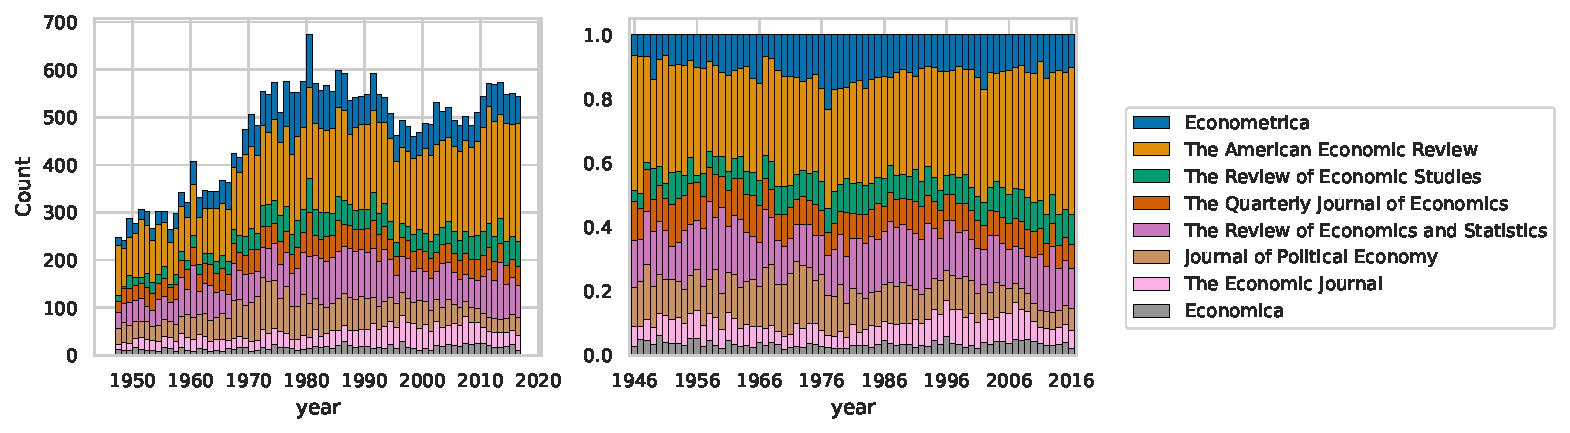
\includegraphics[width=\textwidth]{src/journals.pdf}
  \caption[Number of documents per journal and year]{These two plots represent the number of documents in the dataset divided by year and journal. On the left, the absolute number is reported, while on the right the same data is reported normalized by year.}
  \label{fig:journals}
\end{figure}

Figure \ref{fig:journals} shows the absolute and relative composition of the final dataset disaggregated by journal and year.
The most represented journal is the AER, and it is possible to observe the slowdown in publication described by \textcite{ellison2003,card2013}.

\section{Model selection and validation}
The hSBM algorithm is sensitive to the initial conditions, provided as random seed. For this reason three different random seeds are given to the algorithm and the three outputs are compared.

\begin{table}[tb]
\centering
\caption[Number of groups per level and seed]{Number of groups (both words and documents) in each level of the hierarchy for each random seed}
\label{tab:levels}
\begin{tabular}{l|rrrrrrrr}
\toprule
level &     0 &     1 &    2 &   3 &  4 &     5 &     6 \\
seed &       &       &      &     &    &       &       \\
\midrule
1000 &  7721 &  1418 &  137 &  21 &  3 &     2 &   \\
1001 &  7758 &  1350 &  253 &  30 &  4 &   &   \\
1002 &  9055 &  1774 &  218 &  31 &  5 &     4 &     2 \\
\bottomrule
\end{tabular}
\end{table}


Table \ref{tab:levels} shows the instability of the model: the number of levels in the hierarchy is different (but similar) for each random seed, and so is the number of groups (composed by either documents or words) at each level.
On the other hand, for the first five levels of the hierarchy (0 to 4) the magnitude of the number of levels is the same independently of the random seed (and so they describe the model at the same scale).

For the reasons stated above, the level of the hierarchy at the scale of interest is the level 3.

\begin{figure}[tb]
  \centering
  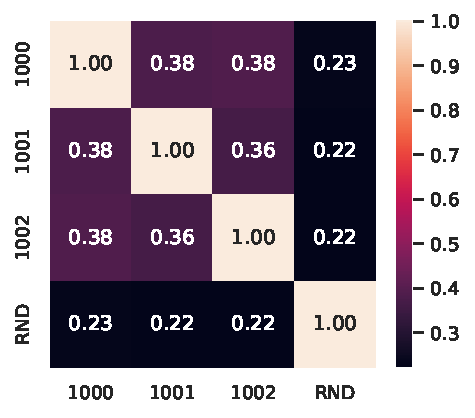
\includegraphics[width=3.5in]{src/mi.pdf}
  \caption[Mutual Information for the level of interest]{Normalized mutual information for the three level 3 partitions and a random control partition (RND)}
  \label{fig:mi}
\end{figure}

To verify that the similarity is not only in the magnitude but also in the composition of the groups a null-model is generated. Focusing on the level of interest, the average number of words-groups and documents-groups are computed. Then, words (documents) are randomly divided in such number of groups. The resulting partitions (the null-model and the three topic models) are compared using the Normalized Mutual Information. As shown in figure \ref{fig:mi} the mutual information between the three topic models is higher (.36-.38) then the mutual information between one of the topic models and the control partition (.22-.23). This is a strong hint that the three models recognize some kind of structure (the topics) and their similarity is not a coincidence.

\begin{table}[tb]
\centering
\caption[Model and level entropy]{The table reports the entropy of the inferred partition for the whole model and for the level of intersed, per each random seed (lower is better)}
\label{tab:entropy}
\begin{tabular}{rrr}
\toprule
 seed &  Model Entropy &  Level 3 Entropy \\
\midrule
 1000 &   9.946873e+07 &     7.764964e+06 \\
 1001 &   9.928597e+07 &     9.217477e+06 \\
 1002 &   9.795245e+07 &     8.391116e+06 \\
\bottomrule
\end{tabular}
\end{table}


At this point it is necessary to chose one of the three models to analyse in details. The algorithm chosen (hSBM) provides a measure of the goodness-of-fit for both the complete hierarchy and each level. The metric is the entropy of the partition inferred, which, qualitatively, express how much information is needed to describe the model given the partition. So, lower the entropy more informative on itself is the partition.

From table \ref{tab:entropy}, the model with random seed 1002 is the one with the lower entropy of the hierarchy, while the model 1000 is the one with the lower entropy for the level we are interested in (and it is also the one with the smaller amount of groups in that level, see table \ref{tab:levels}). Since in this work I don't exploit the presence of a full hierarchy, but I analyse only a single level, the choice of the model is driven by the entropy of the level, and so the model 1000 is chosen, and it is the only one considered in the following section.

\section{Interpreting the model}
The chosen partition is composed by 9 groups of documents and 12 topics (or groups of words).
To interpret the model it is useful to give a name to each topic and group.

\begin{table}[tb]
\centering
\caption[Groups]{The nine documents-group and the twenty most frequent words in each of them}
\label{tab:groups}
\begin{tabularx}{\hsize}{lY}
\toprule
         Applied Microeconomics &                             educ, household, children, women, health, child, birth, parent, insur, job, men, black, unemploy, male, cohort, femal, white, hour, fertil, student \\
Applied Microeconomics - Labour &                                household, educ, unemploy, student, job, hous, hour, panel, citi, women, union, insur, dummi, yes, children, health, score, labour, skill, shock \\
                    Game Theory &                     game, player, payoff, bid, belief, lemma, buyer, auction, seller, equilibria, signal, princip, bidder, bargain, match, nash, experiment, learn, pair, finit \\
        Industrial Organization &                             entri, vote, advertis, capac, buyer, bid, voter, plant, parti, monopoli, seller, auction, regul, innov, game, locat, monopolist, retail, rent, sell \\
    International - Development &                 export, union, agricultur, foreign, farm, manufactur, war, plant, domest, patent, skill, unemploy, inflat, educ, soviet, land, credit, million, labour, compani \\
                         Labour &                                 job, unemploy, hous, household, match, educ, skill, labour, citi, shock, rent, insur, innov, union, home, hire, subsidi, poverti, credit, panel \\
         Macro - Trade - Growth &                    export, tariff, foreign, domest, labour, manufactur, unemploy, shock, inflat, protect, union, household, credit, gdp, cycl, plant, home, nomin, debt, capita \\
                 Macroeconomics &             inflat, shock, debt, forecast, bond, credit, foreign, nomin, liquid, borrow, currenc, cycl, loan, domest, investor, corpor, unemploy, portfolio, household, volatil \\
                    Mathematics & asymptot, matrix, lemma, converg, finit, sequenc, moment, likelihood, covari, densiti, stochast, shock, path, convex, uniform, instrument, root, volatil, equilibria, portfolio \\
\bottomrule
\end{tabularx}
\end{table}


To label the groups the occurrences of each word in each document of the group are summed together, then the most frequent words in the group are used to get a general sense of the group (table \ref{tab:groups}). Moreover, considering this sum as a single document, the most similar documents (using the cosine similarity) to the group as whole are also listed (see table \ref{tab:papers} in appendix).

\begin{table}[tb]
\centering
\caption[Topics]{The twelve topics (words-group) and the twenty most frequent words for each of them}
\label{tab:topics}
\begin{tabularx}{\hsize}{lY}
\toprule
                 Credit &                     inflat, credit, spend, tariff, borrow, loan, budget, home, corpor, compani, war, nomin, capita, reform, portfolio, fiscal, cash, intens, equiti, residu \\
           Econometrics & shock, panel, matrix, forecast, liquid, robust, transact, volatil, avers, volum, gdp, behaviour, schedul, profil, inventori, transform, frequenc, mathemat, baselin, global \\
    Econometrics - Time &                   household, hour, cycl, instrument, day, rent, week, longrun, compens, expans, gap, slope, subsidi, moment, fluctuat, persist, top, old, access, communiti \\
            Game Theory &                  game, player, payoff, bid, seller, auction, uniform, cooper, bidder, nash, network, round, switch, win, conflict, monitor, lotteri, axiom, coalit, sustain \\
Industrial Organization &                     entri, buyer, bargain, locat, vote, capac, extern, surplus, parti, regul, sell, her, median, monopoli, buy, distanc, experiment, charg, voter, advertis \\
                 Labour &                 unemploy, labour, union, manufactur, skill, agricultur, innov, land, food, farm, mobil, equip, oil, professor, cit, enterpris, propens, mine, soviet, rural \\
         Macroeconomics & export, foreign, debt, domest, bond, investor, currenc, macroeconom, gold, recess, treasuri, machin, matur, lender, phillip, keyn, boom, inflationari, devalu, intermediari \\
            Mathematics &         lemma, equilibria, path, converg, learn, belief, signal, asymptot, likelihood, simul, rank, heterogen, finit, sequenc, pair, stochast, densiti, transit, row, endow \\
              Microdata &                                 educ, job, hous, insur, student, dummi, health, children, women, citi, yes, men, black, parent, white, score, status, child, occup, employe \\
             Production &              plant, patent, transport, retail, south, electr, negoti, farmer, partner, entrant, barrier, pollut, crop, divers, fuel, coal, invent, collus, southern, affili \\
             StopWords1 &      match, princip, post, option, agreement, scheme, pool, length, mix, format, attain, connect, ineffici, attract, anticip, largest, exclus, conduct, hypothes, threshold \\
             StopWords2 &                       six, exhibit, systemat, notion, constitut, invers, michael, remov, said, him, via, princeton, modifi, unchang, text, confirm, preced, sup, seek, goal \\
\bottomrule
\end{tabularx}
\end{table}


For the topics (the groups composed by words), instead, the most frequent words in the corpus are listed for each topic \ref{tab:topics}. \textit{StopWords} are the two topics which regroup words with different meanings and which does not bring a semantic insight.

\begin{table}[tb]
\centering
\caption[Groups-Topics]{The composition of each group as a mixture of topics. Only the topics which represent at least 10\% of the group are listed}
\label{tab:gt}
\begin{tabularx}{\hsize}{lY}
\toprule
         Applied Microeconomics &                                                        0.34*Microdata + 0.14*Econometrics~-~Time + 0.11*StopWords1 + ... \\
Applied Microeconomics - Labour &                                                        0.19*Microdata + 0.14*Econometrics~-~Time + 0.12*StopWords1 + ... \\
                    Game Theory &                               0.23*Mathematics + 0.18*Game~Theory + 0.14*StopWords1 + 0.11*Industrial~Organization + ... \\
        Industrial Organization &     0.17*Industrial~Organization + 0.14*StopWords1 + 0.13*Mathematics + 0.12*StopWords2 + 0.11*Econometrics~-~Time + ... \\
    International - Development &                                         0.17*StopWords1 + 0.15*StopWords2 + 0.15*Credit + 0.12*Econometrics~-~Time + ... \\
                         Labour &                   0.16*Mathematics + 0.13*StopWords1 + 0.12*Econometrics~-~Time + 0.11*Microdata + 0.11*StopWords2 + ... \\
         Macro - Trade - Growth &                      0.18*Credit + 0.13*StopWords1 + 0.12*StopWords2 + 0.12*Econometrics~-~Time + 0.10*Mathematics + ... \\
                 Macroeconomics &  0.17*Credit + 0.13*Econometrics + 0.13*Mathematics + 0.13*StopWords1 + 0.13*StopWords2 + 0.11*Econometrics~-~Time + ... \\
                    Mathematics &                                           0.38*Mathematics + 0.14*Econometrics + 0.11*StopWords1 + 0.11*StopWords2 + ... \\
\bottomrule
\end{tabularx}
\end{table}


Once both groups and topics are labelled, it is possible to express a group as a combination of topics, as in table \ref{tab:gt}\footnote{This representation suggests an interesting thought. Science evolve also by recombining older ideas, and we are in fact hypothesizing, by using this model, that the same group of words has a different meaning if used in different context. Algorithm, like LDA, with a single intermediate layer provide a similar insight allowing each word to belong to different topics, and more than one topic to be present in a single document.}.

This is, obviously, only one possible strategy to label topics and groups, but it is the most common used, since it does not require additional data.

\begin{figure}[tb]
  \centering
  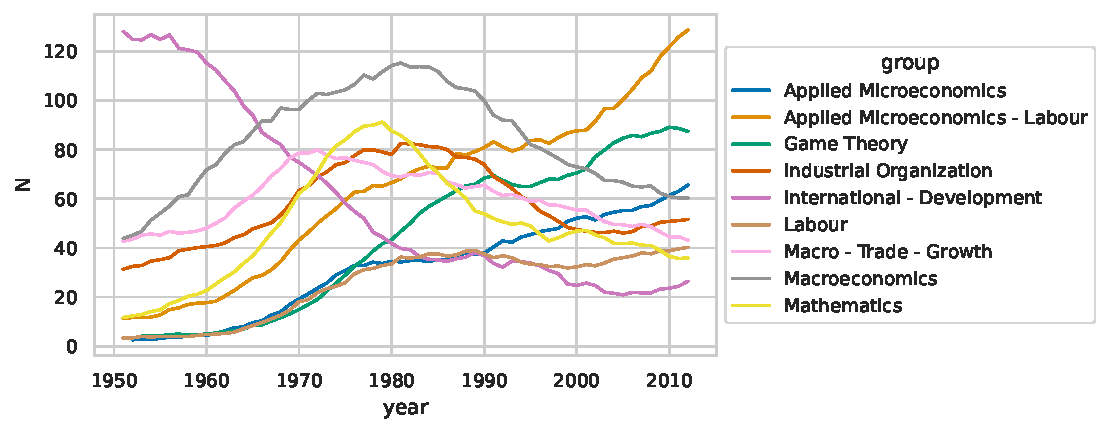
\includegraphics[width=\textwidth]{src/groups.pdf}
  \caption[Groups]{Number of documents in each group during time. Smoothed with a 10-year rolling average}
  \label{fig:groups}
\end{figure}

\begin{figure}[tb]
  \centering
  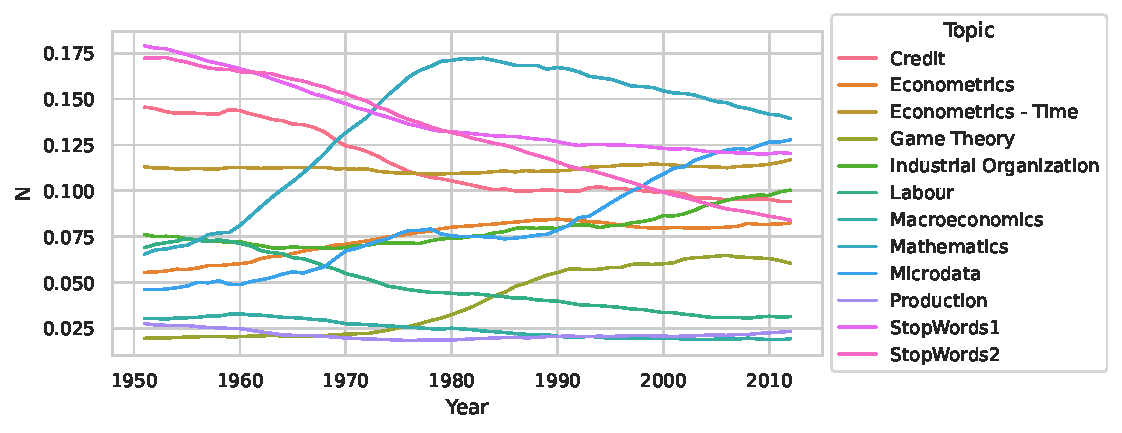
\includegraphics[width=\textwidth]{src/topics.pdf}
  \caption[Topics]{Prevalence of each topic during time. Smoothed with a 10-year rolling average}
  \label{fig:topics}
\end{figure}

Finally, the evolution of groups and topics in time is reported in figure \ref{fig:groups} and \ref{fig:topics} (the plot report the graph smoothed with a 10-years moving average).

\subsection{The empirical turn}
Looking at the groups over time plot (figure \ref{fig:groups}) some very noticeable trends appears.

First the group labelled \textit{International - Development} (which includes \textit{union}, \textit{war} and \textit{soviet} among the most frequent words) is by far the most prevalent group at the beginning of the period and rapidly reduces its presence in the following years. This can be linked (but a more careful look is needed) to the progressive disappearing of the (original) Keynesianism and the classical political economy, in addition to the lost of interest in planned economies.

The centre of the period (the seventies and the eighties) are characterized by the peak of \textit{Macroeconomics} and \textit{Mathematics}, which is reasonable to trace it back to the golden period of neo-Keynesian and neoclassical economics.

Three groups show a growth from the beginning to the end of the time span: \textit{Game Theory} and the two \textit{Applied Microeconomics}. The top five words of the group \textit{Game Theory} (\textit{game}, \textit{player}, \textit{payoff}, \textit{bid}, \textit{belief}) can also describe the kind of laboratory experiment used in behavioural economics, another applied field.

Similar considerations emerge, with less clarity, by analysing the topics (figure \ref{fig:topics}). Particularly the topic labelled \textit{Microdata} (which most frequent words recall micro-econometric studies) shows the strongest growth in the period.

Those observations allow answering positively to the question "There has been an empirical turn in economics and is it possible to measure it?" (which, to be honest, has been already done in literature with other methods).

\subsection{Mainstream pluralism?}
The way the model has been presented tells very little on the other focal point of the study: the mainstream pluralism hypothesis.
The empirical turn described above has been described as a condition that facilitate fragmentation and specialization \parencite{cedrini2018,backhouse2017}, but on its own is only a clue.

\begin{table}[tb]
\centering
\caption[Subgroups]{The numbers of groups in the more detailed level of the hierarchy for each group in the level of interest}
\label{tab:subgroups}
\begin{tabular}{lr}
\toprule
Applied Microeconomics - Labour &  11 \\
Macro - Trade - Growth          &   8 \\
Labour                          &   7 \\
Game Theory                     &   6 \\
Industrial Organization         &   6 \\
Macroeconomics                  &   6 \\
International - Development     &   4 \\
Mathematics                     &   4 \\
Applied Microeconomics          &   2 \\
\bottomrule
\end{tabular}
\end{table}


The hierarchical nature of the model allows counting the subgroups for each group (table \ref{tab:subgroups}) but the results are not interesting.
The numerosity of the subgroups does not appear to be linked neither with the more applied fields, nor with the time in which a group reached its peak.

It is time to take a step back, to lose the model from sight and to try to refrain the question in a more concrete way. Pluralism is the coexistence of different programmes, each with a different goal and, it is reasonable to assume, slightly different lexicons. So, in a pluralistic period the number of different words used should be higher than in a homogeneous period.

\begin{figure}[tb]
  \centering
  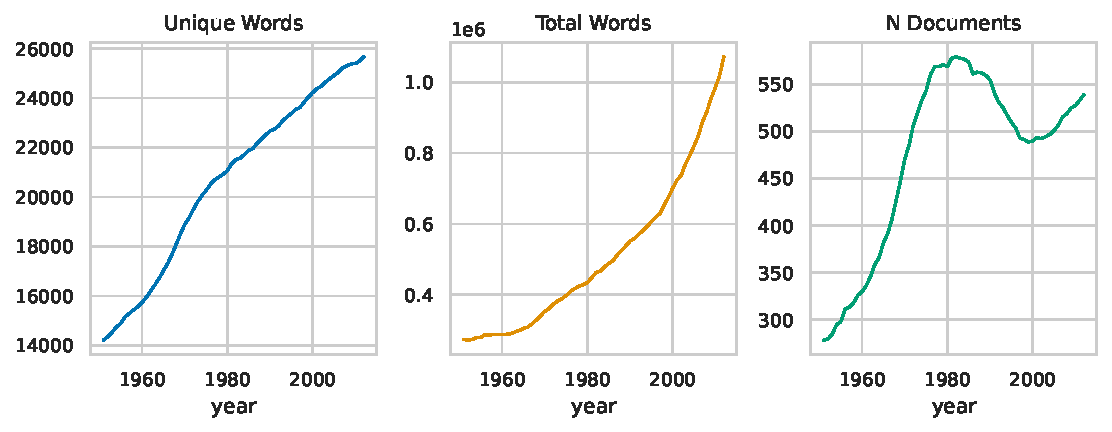
\includegraphics[width=\textwidth]{src/uwords.pdf}
  \caption[Unique Words]{From left to right: number of unique words per year in the sample; total number of words per year in the sample; number of documents per year in the sample}
  \label{fig:uwords}
\end{figure}

To illustrate this idea, the number of unique words used in each year is measured, and then it is compared to the number of papers in the sample and the total words used (i.e. the total length of the cleaned papers published in a year). Figure \ref{fig:uwords} summarize the comparison.

The number of the unique words used grows from the beginning of the sample and since the eighties it grows faster than the number of newly published documents. This means that the probability that a new document introduces a new word (for example because a new subfield has reached the status to be accepted in the top journals) is increasing too.

On the other hand, the total number of words published is increasing way faster than the number of unique words, because of the progressive increment in length of the papers. This suggests that the increased lexical variety is not a matter of diversification, by a necessary by-product of longer articles.

Using these data, I am not able to see a way to exclude one of the two explanations.

To summarize, I have not found in this topic model a good instrument to measure the (eventual) advent of a new mainstream pluralism. This can be the consequence of the specific algorithm used or a signal that the research question has to be rephrased in a more theory-aware way.

\section{Limitations}
This study is a work in progress, and probably cannot reach a mature stage without a huge multidisciplinary effort.

Here and there, a lot of arbitrary choices and unrefined step are present (explicitly or not).
Some of them can be resolved with a lot of time, good relations with commercial providers of databases and/or a high performance cluster (a very fast computer).
Some others open the windows on huge gaps in literature.

I will discuss some of them.

The idea of focusing on the top journals as a proxy for the mainstream convinces me. But which are the top journals is debatable.
If only a smaller time period is going to be considered, approximately from the eighties until today, the Top5 can be an exhaustive group. But the equilibria in the discipline in the previous decades were less defined.
Moreover, the very choice to use textual data rather than, for example, bibliometric ones is not written in stone.

There are at least three steps which can benefit by a robustness check: the cleaning of the dataset, the inference of the model and its interpretation.

The choice of stemming the dataset is arbitrary and should be checked if the alternatives (lemmatization, embedding and doing nothing) impact the model inferred.
Similarly, the strategy used to reduce the size of the vocabulary, cutting the words presents in many of few documents, is only one of the possibility, and maybe not the best one \parencite{gerlach2019}.

Allowing that inferring a topic model is the right way to approach this problem, there is not a consensus in literature in which algorithm perform better and, maybe more important, how to compare them \parencite[a recent and rare attempt is][]{shi2019}. I still believe that the limitations of LDA, particularly the need to determine a priori the number of topic, require pivoting to some more modern algorithms. Which is still an open question.

Even testing more algorithms, how should they be interpreted if the proposed partitions are significantly different one from the others?

At very least, the exercise of interpreting the resulting model should be repeated for each of the inferred models (with the three different random seed used) to see what is consistent across them and what, instead, change\footnote{Everything needed for this exercise is available in the folder \texttt{out} of the online repository.}

Finally, the labels given to the topics and the groups are subjective, and the method chosen is dictated more by the data at disposition than by some fine reasoning.
JSTOR is a fantastic resource to get the word count of many (but not all!) journals\footnote{But it does not provide the full text, which can be a useful resource for more advanced machine learning models.}, but it does not keep track of the citations received by a work, or the JEL codes attributed to it. Moreover, there is not a public database that relates the JSTOR identifier, with the Scopus one\footnote{A lot of the older document are missing from Scopus. As consequence, every study that relies on it to get bibliometric data, even just to identify the most relevant paper in a cluster, is constrained in the time period that can be studied.} or the EconLit one\footnote{The EconLit database associates to every record its JEL codes. But there are some different taxonomies of JEL codes for different periods, the last big update happened in 1990 \parencite{cherrier2017}, without a clear way to convert one in another.}, making the operation of mixing metadata from different sources really difficult and time-consuming.
Two other strategies to interpret the groups have been discarded for this reason: label each group with the most frequent JEL Codes, and characterize each group with the most cited documents in it.

\section{What's next?}
I can suggest four direction in which this work can continue.

The first one is to explore another finer-grained level of the hierarchy to look for specific subfields described in literature as part of the mainstream pluralism \parencite[§1]{davis2006}, and observe their evolution through time.

The second one is to substitute hSBM with another algorithm (maybe BERTtopic), and observe what will change and what not.

The third one is to enhance the JSTOR database with citations data (from Scopus) and the JEL codes of the articles (from EconLit). Doing so requires to limit the time span (going back no later than 1980) and a lot of time, probably provided by master students for their thesis.

The last one is probably the most important and most radical: forget about this work, doing a deeper qualitative study to highlight the very own characteristic of mainstream pluralism and translate them into quantitative question.
There is a debate in the part of the digital humanities' community who studies history of ideas: is it better to use complex models to highlight some general features that are not observable by a human's eye (like in this work), or is it better to formulate more precise questions and try to measure some very specific features (like I did in \textcite{babbiotti2022})?
I am inclined to the second approach, mostly because the data manipulated in this kind of studies are rarely high quality data, and more complex the algorithm more probable is that the noise of the data is transformed in a feature of the model. The possible side effect of simpler and understandable measures are easier to be spotted, allowing for a more conscious management of the noise in the data (like a poor OCR, or an imperfect coupling between two data sources).

Unfortunately, at the time of writing, I have not in mind a characterization of the mainstream pluralism (or alternatively of what makes a research programme "post-neoclassical") clear enough to hypothesize some measurable proxies for it. But it can be the topic of another paper.

\section*{Acknowledgments}
This paper is a (very) revised version of my master thesis, which benefitted from the excellent guidance of my supervisors, Michele Caselle, Mario Cedrini e Alessandra Durio, and the useful critiques provided by Matteo Osella.
This work would not have been possible without the (computational) help provided by Diletta Abbonato in the exploratory phase, the, often ignored, advices from Carlo Debernardi, and the freedom to pursue secondary projects during the PhD granted me by Eugenio Caverzasi (and his support).
The revisions of the various versions of this manuscript have taken advantage of Alice Re's scrupulousness and helpfulness.
Finally, I want to thank the whole DR2 community for the numerous stimuli in continuing working on quantitative history of the ideas and particularly Paolo Babbiotti, and Eugenio Petrovich, who, in a cold January in Rome, taught me how to write an Acknowledgments section.

\clearpage
\begin{refcontext}[sorting=nyt]
  \printbibliography
\end{refcontext}
\clearpage

\begin{appendices}
  \section{Additional tables}
  \begin{landscape}
    \begin{xltabular}[p]{\hsize}{sYsrs}

\caption[Representative papers]{The five papers most representative of each group, measured by the cosine similarity with the word count in the topic as whole}
\label{tab:papers} \\ \toprule \endhead \hline \multicolumn{5}{r@{}}{\textit{continues on  next page}}\\ \hline \endfoot \hline \endlastfoot


         Applied Microeconomics &                                                 Alimony Rights and Intrahousehold Allocation of Resources: Evidence from Brazil &                                              Marcos A. Rangel & 2006 &                   The Economic Journal \\
         Applied Microeconomics &                                                    Household and Economy: Toward a New Theory of Population and Economic Growth &                                                  Marc Nerlove & 1974 &           Journal of Political Economy \\
         Applied Microeconomics &                                                                                       Child Quality and the Demand for Children &                                             Dennis N. De Tray & 1973 &           Journal of Political Economy \\
         Applied Microeconomics &                                                                                                        CONSUMPTION AND CHILDREN &                                 Martin Browning, Mette Ejrnæs & 2009 & The Review of Economics and Statistics \\
         Applied Microeconomics & Differences in Education and Earnings Across Racial and Ethnic Groups: Tastes, Discrimination, and Investments in Child Quality &                                             Barry R. Chiswick & 1988 &     The Quarterly Journal of Economics \\
Applied Microeconomics - Labour &                                                   The Macroeconomic Implications of Rising Wage Inequality in the United States & Jonathan Heathcote, Kjetil Storesletten, Giovanni L. Violante & 2010 &           Journal of Political Economy \\
Applied Microeconomics - Labour &                                                                     Relative Wage Movements and the Distribution of Consumption &                             Orazio Attanasio, Steven J. Davis & 1996 &           Journal of Political Economy \\
Applied Microeconomics - Labour &                                            Unemployment Risk and Precautionary Wealth: Evidence from Households' Balance Sheets &      Christopher D. Carroll, Karen E. Dynan, Spencer D. Krane & 2003 & The Review of Economics and Statistics \\
Applied Microeconomics - Labour &                                                 Financial Wealth, Consumption Smoothing and Income Shocks Arising from Job Loss &                      Hans G. Bloemen, Elena G. F. Stancanelli & 2005 &                              Economica \\
Applied Microeconomics - Labour &                                                                               Wage Risk and Employment Risk over the Life Cycle &                   Hamish Low, Costas Meghir, Luigi Pistaferri & 2010 &           The American Economic Review \\
                    Game Theory &                                                                          EFFICIENCY IN GAMES WITH MARKOVIAN PRIVATE INFORMATION &                                 Juan F. Escobar, Juuso Toikka & 2013 &                           Econometrica \\
                    Game Theory &                                                            Ten Little Treasures of Game Theory and Ten Intuitive Contradictions &                              Jacob K. Goeree, Charles A. Holt & 2001 &           The American Economic Review \\
                    Game Theory &                                                                                          Global Games and Equilibrium Selection &                                 Hans Carlsson, Eric van Damme & 1993 &                           Econometrica \\
                    Game Theory &                                                                                                              Large Robust Games &                                                    Ehud Kalai & 2004 &                           Econometrica \\
                    Game Theory &                                                                    Endogenous Games and Mechanisms: Side Payments among Players &                              Matthew O. Jackson, Simon Wilkie & 2005 &         The Review of Economic Studies \\
        Industrial Organization &                                                                                               Industrial Economics: An Overview &                                           Richard Schmalensee & 1988 &                   The Economic Journal \\
        Industrial Organization &                                                                                             The Product as an Economic Variable &                                          Edward H. Chamberlin & 1953 &     The Quarterly Journal of Economics \\
        Industrial Organization &                                                                             The A \& P Case: A Study in Applied Economic Theory &                                                 M. A. Adelman & 1949 &     The Quarterly Journal of Economics \\
        Industrial Organization &                                                                                                      Entry Barriers in Politics &                                                Gordon Tullock & 1965 &           The American Economic Review \\
        Industrial Organization &                                                                          Surveys of Applied Economics: Price Behaviour of Firms &                                             Aubrey Silberston & 1970 &                   The Economic Journal \\
    International - Development &                                                                                                A Review of Economic Development &                                               W. Arthur Lewis & 1965 &           The American Economic Review \\
    International - Development &                         The Relation Between Home Investment and External Balance in the Light of British Experience, 1945-1955 &                                                 Ragnar Nurkse & 1956 & The Review of Economics and Statistics \\
    International - Development &                                                  Mexican Economic Policy in the Post-War Period: The View of Mexican Economists &                                                Leopoldo Solís & 1971 &           The American Economic Review \\
    International - Development &                                    Yugoslav Economic Policy in the Post-War Period: Problems, Ideas, Institutional Developments &                                                 Branko Horvat & 1971 &           The American Economic Review \\
    International - Development &                                                                                          The Economics of Development: A Survey &                                                Nicholas Stern & 1989 &                   The Economic Journal \\
                         Labour &                                                                               Wage Risk and Employment Risk over the Life Cycle &                   Hamish Low, Costas Meghir, Luigi Pistaferri & 2010 &           The American Economic Review \\
                         Labour &                                                                                  Markets with Search Friction and the DMP Model &                                             Dale T. Mortensen & 2011 &           The American Economic Review \\
                         Labour &                                                                                     On-the-Job Search and Precautionary Savings &                                                   JEREMY LISE & 2013 &         The Review of Economic Studies \\
                         Labour &                                                                                                  Unemployment, Vacancies, Wages &                                                 Peter Diamond & 2011 &           The American Economic Review \\
                         Labour &                                                                                         Business Cycles and Labor-Market Search &                                              David Andolfatto & 1996 &           The American Economic Review \\
         Macro - Trade - Growth &                         The Relation Between Home Investment and External Balance in the Light of British Experience, 1945-1955 &                                                 Ragnar Nurkse & 1956 & The Review of Economics and Statistics \\
         Macro - Trade - Growth &                                                                                    Countercyclical Weapons for the Open Economy &                                                 Edward Marcus & 1954 &           Journal of Political Economy \\
         Macro - Trade - Growth &                                                                                  Growth Strategies in Semi-Industrial Countries &                                                  Bela Balassa & 1970 &     The Quarterly Journal of Economics \\
         Macro - Trade - Growth &                                                Increasing International Economic Interdependence: The Implications for Research &                            C. Fred Bergsten, William R. Cline & 1976 &           The American Economic Review \\
         Macro - Trade - Growth &                                                       "Availability" and Other Influences on the Commodity Composition of Trade &                                              Irving B. Kravis & 1956 &           Journal of Political Economy \\
                 Macroeconomics &                                                           A Sample Survey of the Commission on Money and Credit Research Papers &                                         Martin Bronfenbrenner & 1963 & The Review of Economics and Statistics \\
                 Macroeconomics &                                                                                                  The Conduct of Monetary Policy &                                              Charles Goodhart & 1989 &                   The Economic Journal \\
                 Macroeconomics &                                                                                           Recent Developments in Macroeconomics &                                               Stanley Fischer & 1988 &                   The Economic Journal \\
                 Macroeconomics &                                                     Market Sentiment and Macroeconomic Fluctuations under Pegged Exchange Rates &                                         Pierre-Richard Agénor & 2006 &                              Economica \\
                 Macroeconomics &                                                                          Development and Implications of Federal Reserve Policy &                                              Walter A. Morton & 1957 &           The American Economic Review \\
                    Mathematics &                                                                          Asymptotic Normality, When Regressors Have a Unit Root &                                               Kenneth D. West & 1988 &                           Econometrica \\
                    Mathematics &                                                                                              Probit with Dependent Observations &                                 Dale J. Poirier, Paul A. Ruud & 1988 &         The Review of Economic Studies \\
                    Mathematics &                                                             Large Sample Properties of Generalized Method of Moments Estimators &                                             Lars Peter Hansen & 1982 &                           Econometrica \\
                    Mathematics &                                                                       Multiple Time Series Regression with Integrated Processes &                              P. C. B. Phillips, S. N. Durlauf & 1986 &         The Review of Economic Studies \\
                    Mathematics &                                                                        TESTING FOR COMMON CONDITIONALLY HETEROSKEDASTIC FACTORS &                                 Prosper Dovonon, Eric Renault & 2013 &                           Econometrica \\


\end{xltabular}

  \end{landscape}

\end{appendices}

\end{document}